\documentclass[preprint,review,3p]{elsarticle}
\usepackage{amsmath}
\usepackage{amssymb}
\usepackage{pgfplots}
\usepackage{tikz}

\begin{document}

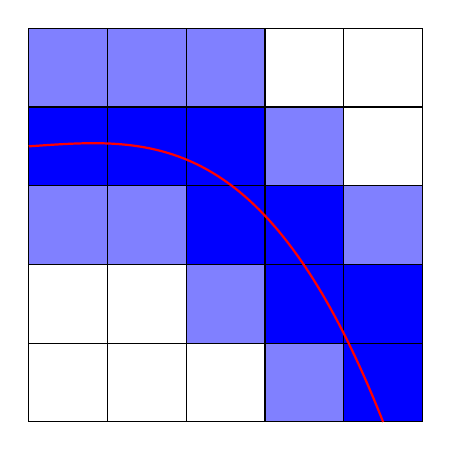
\begin{tikzpicture}
    \fill[white!50] (0,0) rectangle (5,5);
    \fill[blue!100] (0,3) rectangle (1,4);
    \fill[blue!100] (1,3) rectangle (2,4);
    \fill[blue!100] (2,3) rectangle (3,4);
    \fill[blue!100] (2,2) rectangle (3,3);
    \fill[blue!100] (3,2) rectangle (4,3);
    \fill[blue!100] (3,1) rectangle (4,2);
    \fill[blue!100] (4,1) rectangle (5,2);
    \fill[blue!100] (4,0) rectangle (5,1);

    \fill[blue!50] (0,4) rectangle (1,5);
    \fill[blue!50] (1,4) rectangle (2,5);
    \fill[blue!50] (2,4) rectangle (3,5);
    \fill[blue!50] (3,3) rectangle (4,4);
    
    \fill[blue!50] (4,2) rectangle (5,3);
    \fill[blue!50] (0,2) rectangle (1,3);
    \fill[blue!50] (1,2) rectangle (2,3);
    \fill[blue!50] (2,1) rectangle (3,2);
    \fill[blue!50] (3,0) rectangle (4,1);
    \draw[step=1.0,black,thin] (0,0) grid (5,5);
    \draw[red,thick] (4.5,0) .. controls (3,3.8) and (1.5,3.6) .. (0,3.5);
    \end{tikzpicture}

\end{document}